\chapter{System Testing and Evaluation}\label{chap:testingEvaluation}

%\version{v1.11.2015}

\section*{}In this chapter the testing and evaluation of ADD application.


 \section{Graphical user interface testing}
	\begin{enumerate}
		\item Test Case 1:
For this testing there is start button on main screen which opens input screen shown in Figure \ref{fig:Main to Input Screen} and Table \ref{TestCase1}.
\begin{figure}[ht]
\centering
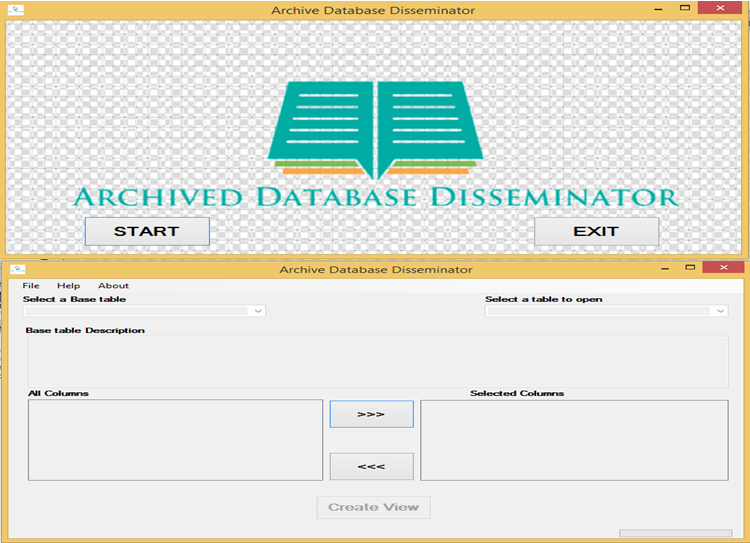
\includegraphics[scale=0.4]{MainToInput}
\caption{Main to Input Screen}
\label{fig:Main to Input Screen}
\end{figure} 

\begin{table}[]
\centering
\begin{tabular}{|l|l|}
\hline
\bfseries Test id          & 1                 \\
\hline
\bfseries Title        & Start Application \\
\hline
\bfseries  Test Steps        & Click start button on main form           \\
\hline
\bfseries Expected Result & Application form displayed         \\
\hline
\bfseries Test Result & PASS \\
\hline                   
\end{tabular}
\caption{TestCase1}
\label{TestCase1}
\end{table}
\item Test Case 2:
\par Now select File option from menu bar and choose Open Archive option from that particular menu of ADD. After this get windows dialogue box for input ".siard" file and form will loaded with selected ".siard" file which is shown in Figure \ref{fig:Selecting .siard File} and Table \ref{TestCase2}.


\begin{figure}[ht]
\centering
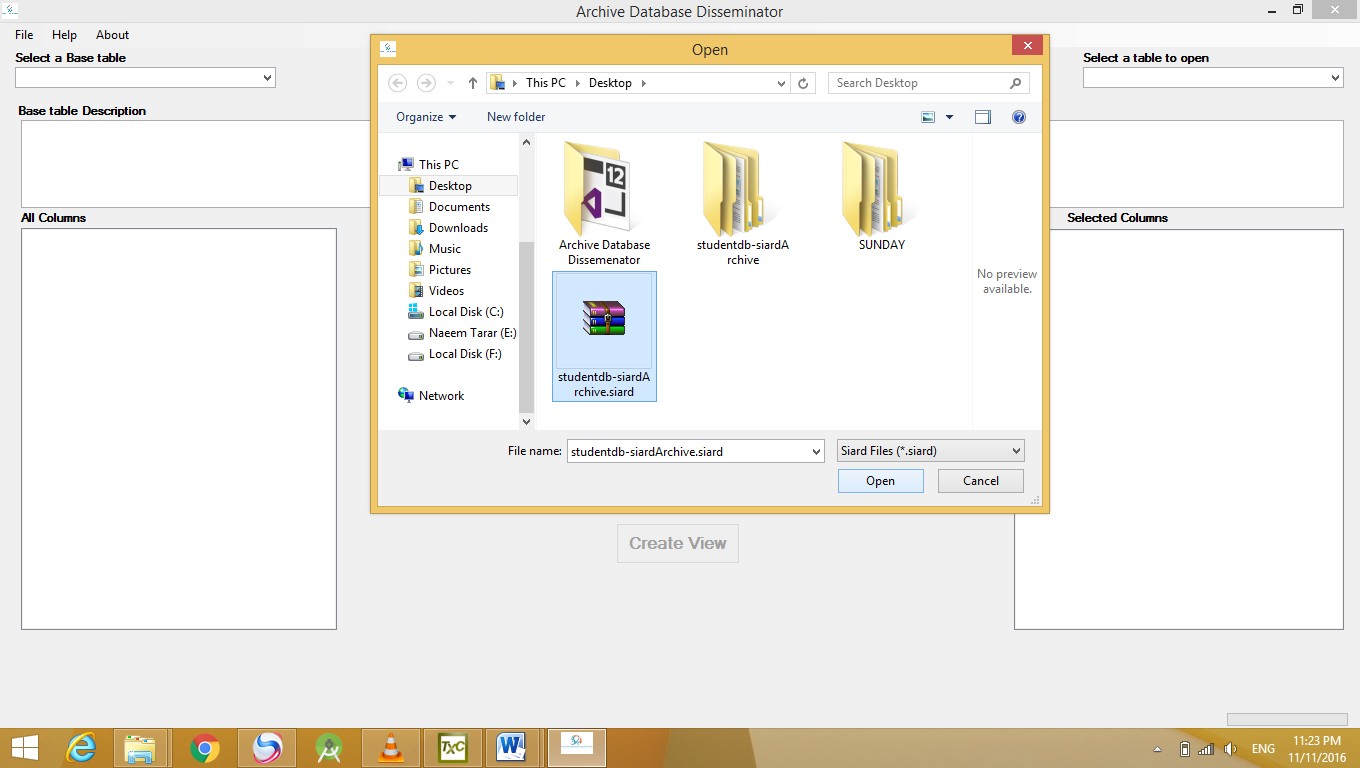
\includegraphics[scale=0.4]{SelectFile}
\caption{Selecting ".siard" File}
\label{fig:Selecting .siard File}
\end{figure} 

\begin{table}[]
\centering
\begin{tabular}{|l|l|}
\hline
\bfseries Test id          & 2                 \\
\hline
\bfseries Title        & Select File \\
\hline
\bfseries  Test Steps        & \makecell{click on file option in menu bar \\ Dialog box open \\Select ".siard" file}          \\
\hline
\bfseries Expected Result & Load ".siard" file         \\
\hline
\bfseries Test Result & PASS \\
\hline                   
\end{tabular}
\caption{TestCase2}
\label{TestCase2}
\end{table}

\par On the basis of selected file can displays these results.
\begin{enumerate}
	\item List of all base tables
	\item Keys of all tables
	\item Description of selected base table
	\item List of all columns
	\item Record of selected table
	\item Search specific record
	\item Search by specific column
	\item Sort the records in columns
	\item Total number of column match and found
\end{enumerate}
which can shown in Figure \ref{fig:Data of selected Table} .
\begin{figure}[ht]
\centering
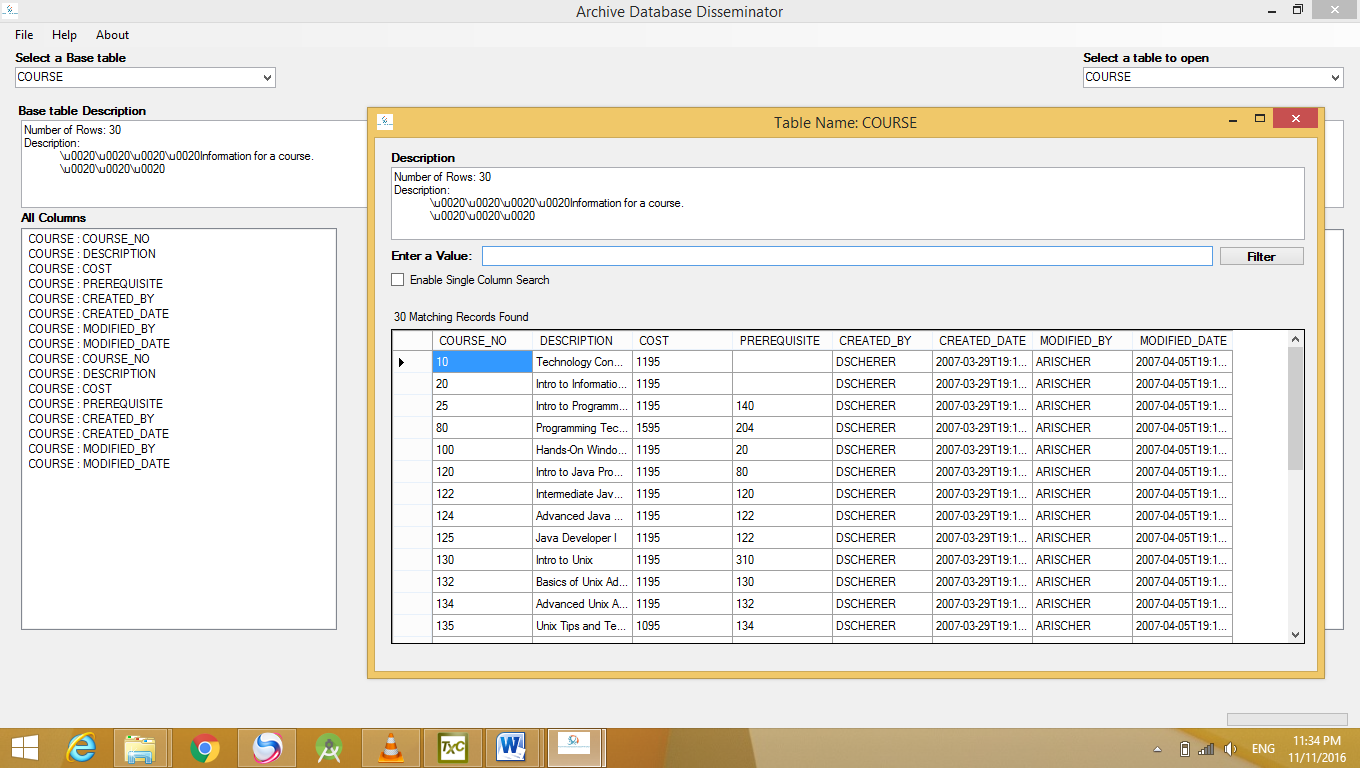
\includegraphics[scale=0.4]{TableDisplay}
\caption{Data of selected Table}
\label{fig:Data of selected Table}
\end{figure}
By selecting specific table now can displays these results: 
\begin{enumerate}
	\item Select specific columns
	\item Create view of selected columns
	\item Description of base table of selected columns
	\item Search specific record
	\item Search by specific column
	\item Sort the records in columns
	\item Totel number of column match and found
\end{enumerate}
which is shown in Figure \ref{fig:View Created of selected columns}.
\begin{figure}[ht]
\centering
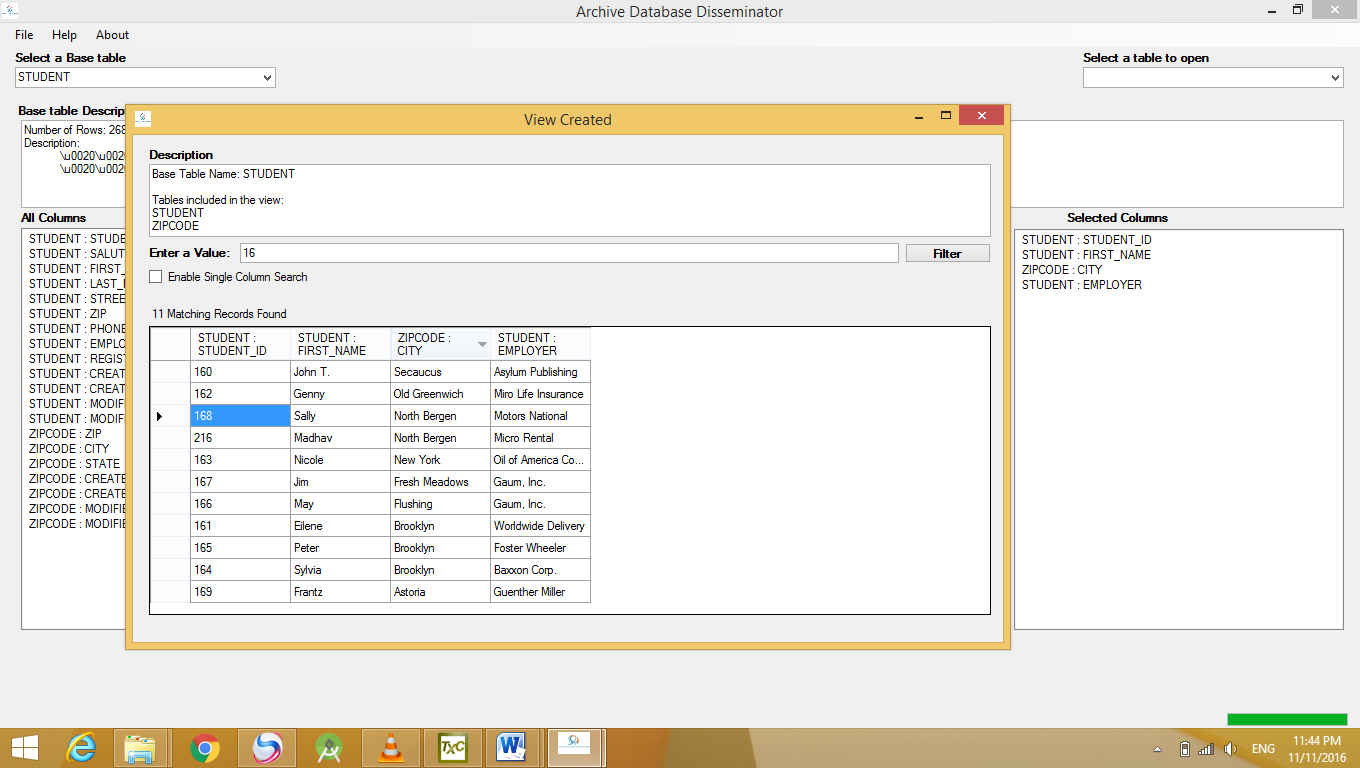
\includegraphics[scale=0.4]{CreateView}
\caption{View Created of selected columns}
\label{fig:View Created of selected columns}
\end{figure}
\item Test Case 3:
If select incorrect file the ADD application give the error message as show in Figure \ref{fig:Incorrect File Selected} and Table \ref{TestCase3}.



\begin{figure}[ht]
\centering
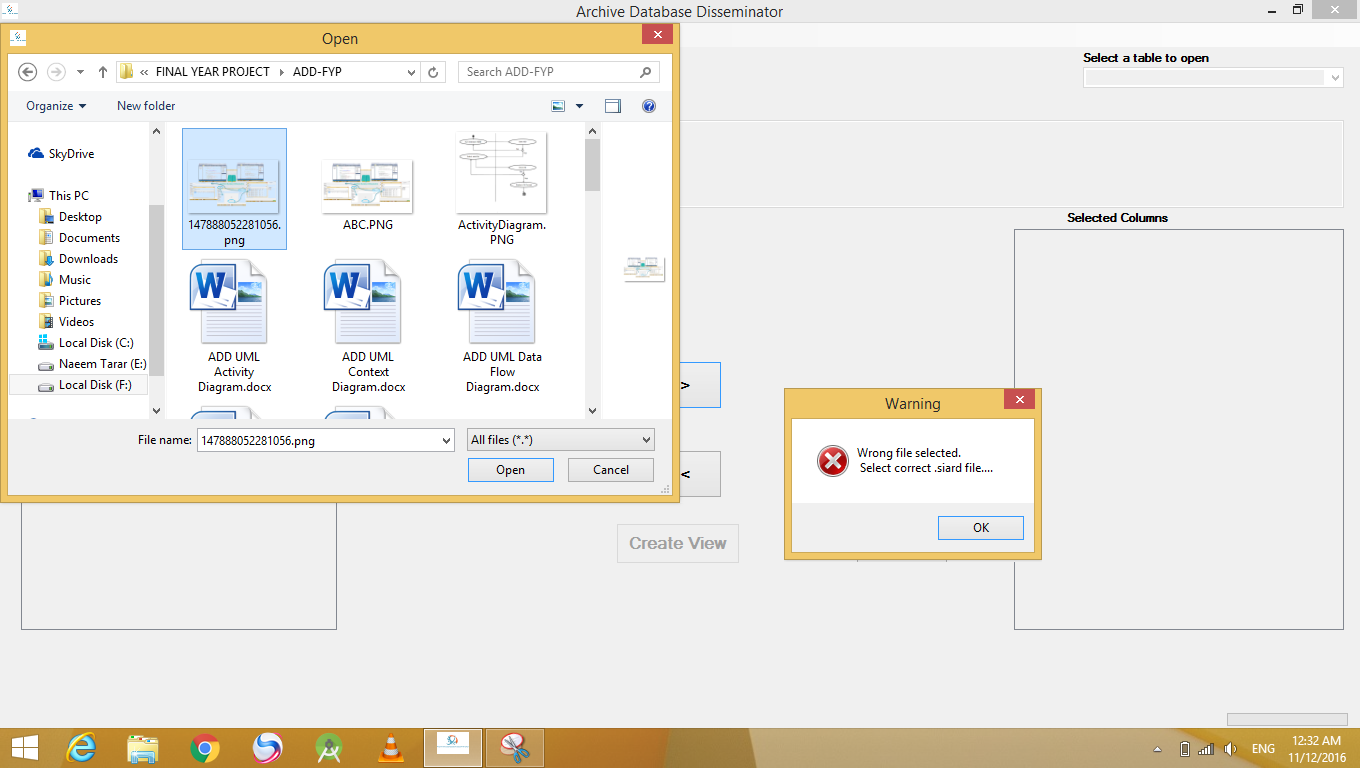
\includegraphics[scale=0.4]{Error}
\caption{Incorrect File Selected}
\label{fig:Incorrect File Selected}
\end{figure}

\begin{table}[]
\centering
\begin{tabular}{|l|l|}
\hline
\bfseries Test id          & 3                 \\
\hline
\bfseries Title        & Select File \\
\hline
\bfseries  Test Steps        & \makecell{click on file option in menu bar \\ Dialog box open \\Select other then ".siard" file}          \\
\hline
\bfseries Expected Result & \makecell{Exception Thorw \\ Error MessageBox displayed}         \\
\hline
\bfseries Test Result & PASS \\
\hline                   
\end{tabular}
\caption{TestCase3}
\label{TestCase3}
\end{table}

\par When user select file other then ".siard" the automatically messagebox is pop up which is basically an error message generated by the application that this extension file cannot loaded in ADD.
	\end{enumerate}
	
  \section{Usability testing}
	The ADD software has compatibility issue with android and IOS platform. It runs only on windows system.
	
	\section{Software performance testing}
	ADD software's performance will shown in Table \ref{Software Performance}.
	\begin{table}[]
\centering
\begin{tabular}{|l|l|}
\hline
\bfseries Run ADD                                 &  1 sec         \\
\hline
\bfseries Load ".siard" file                      &  1 sec       \\
\hline
\bfseries Display columns of selected table       &  1 sec         \\
\hline
\bfseries Display record                          &  1 sec       \\
\hline
\bfseries Create view of selected columns         &  1 sec       \\
\hline
\bfseries Filter the records                      &  1 sec       \\
\hline
\bfseries Sort the columns                        &  1 sec       \\     
\hline
\end{tabular}
\caption{Software Performance}
\label{Software Performance}
\end{table}

	\section{Compatibility testing}
	ADD software can translate in various programming languages by using different tools. This application can develop for other platforms or environments.  
	
	 \section{Exception handling}
	ADD application will throw exception when user select file other then .siard format. These exceptions will show the error message. Which is shown in Figure \ref{fig:Incorrect File Selected}.
	
 \section{Load testing} 
	ADD application not need of installation. In load testing, test ADD with different sizes of ".siard" files like 500KB, 900KB or 2MB. ADD software performance is remain consistent with minor difference in response time shown in Figure \ref{fig:Load the Application}.
	\begin{figure}[ht]
\centering
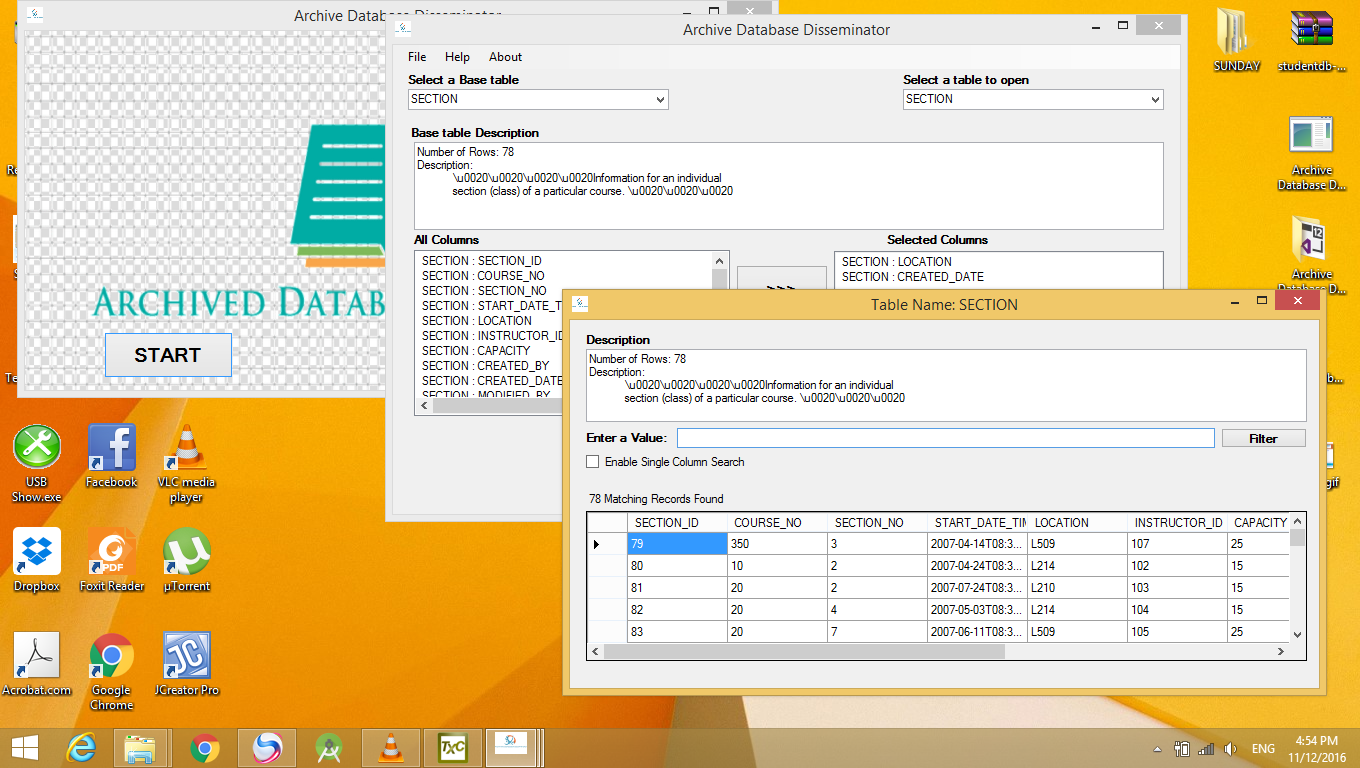
\includegraphics[scale=0.4]{LoadTesting}
\caption{Load the Application}
\label{fig:Load the Application}
\end{figure}

